\documentclass[a4paper, 12pt]{article}
\usepackage{pgfplots}
\usepackage{mathtools}

%% Listings With Code-Styling and Grey Background
\usepackage{float}
\usepackage{listings} 
\usepackage{xcolor}
\usepackage{mdframed}
\usepackage{graphicx}
\definecolor{code-gray}{gray}{0.93}

%% Custom FSM's
\usepackage{tikz}
\usetikzlibrary{automata, positioning, arrows}
\tikzset{very thick, ->, >=stealth', node distance=6cm, every state/.style={thick, fill=gray!10}, initial text=$ $}

%% Automatic Word Formatting
\usepackage{xspace}
\newcommand*{\Vivado}{\textit{Vivado}\xspace} % Italicize Vivado
\newcommand*{\SV}{\textbf{SystemVerilog}\xspace} % Bold SystemVerilog

%% Clickable links in the output PDF
\usepackage{hyperref}
\hypersetup{colorlinks=true, linktoc=all, linkcolor=black}

%% Figure Numbering Within Sections
\let\counterwithout\relax
\let\counterwithin\relax
\usepackage{chngcntr}
\counterwithin{figure}{section}

%% Macros for logic timing diagrams
\newcounter{wavenum}
\setlength{\unitlength}{1cm}
% advance clock one cycle, not to be called directly
\newcommand*{\clki}{
  \draw (t_cur) -- ++(0,.3) -- ++(.5,0) -- ++(0,-.6) -- ++(.5,0) -- ++(0,.3)
    node[time] (t_cur) {};
}
\newcommand*{\bitvector}[3]{
  \draw[fill=#3] (t_cur) -- ++( .1, .3) -- ++(#2-.2,0) -- ++(.1, -.3)
                         -- ++(-.1,-.3) -- ++(.2-#2,0) -- cycle;
  \path (t_cur) -- node[anchor=mid] {#1} ++(#2,0) node[time] (t_cur) {};
}
% \known{val}{length}
\newcommand*{\known}[2]{
    \bitvector{#1}{#2}{white}
}
% \unknown{length}
\newcommand*{\unknown}[2][XXX]{
    \bitvector{#1}{#2}{black!20}
}
% \bit{1 or 0}{length}
\newcommand*{\bit}[2]{
  \draw (t_cur) -- ++(0,.6*#1-.3) -- ++(#2,0) -- ++(0,.3-.6*#1)
    node[time] (t_cur) {};
}
% \unknownbit{length}
\newcommand*{\unknownbit}[1]{
  \draw[ultra thick,black!50] (t_cur) -- ++(#1,0) node[time] (t_cur) {};
}
% \nextwave{name}
\newcommand{\nextwave}[1]{
  \path (0,\value{wavenum}) node[left] {#1} node[time] (t_cur) {};
  \addtocounter{wavenum}{-1}
}
% \clk{name}{period}
\newcommand{\clk}[2]{
    \nextwave{#1}
    \FPeval{\res}{(\wavewidth+1)/#2}
    \FPeval{\reshalf}{#2/2}
    \foreach \t in {1,2,...,\res}{
        \bit{\reshalf}{1}
        \bit{\reshalf}{0}
    }
}

% \begin{wave}[clkname]{num_waves}{clock_cycles}
\newenvironment{wave}[3][clk]{
  \begin{tikzpicture}[draw=black, yscale=.7,xscale=1]
    \tikzstyle{time}=[coordinate]
    \setlength{\unitlength}{1cm}
    \def\wavewidth{#3}
    \setcounter{wavenum}{0}
    \nextwave{#1}
    \foreach \t in {0,1,...,\wavewidth}{
      \draw[dotted] (t_cur) +(0,.5) node[above] {t=\t} -- ++(0,.4-#2);
      \clki
    }
}{\end{tikzpicture}}

%$ Specific Line Breaks
% See https://tex.stackexchange.com/questions/26174/ for details
\usepackage[british]{babel} 

%% Page Margins
\usepackage[margin=1.00in]{geometry}

% Beginning of Document
\begin{document}
\counterwithin{lstlisting}{section} % Listings are numbered within sections
% Title
\title{ECE 440 - Project \#2}
\author{Collin Heist}
\date{\today}
\maketitle

% Table of Content and Listings
\pagenumbering{roman}
\tableofcontents
\renewcommand{\listfigurename}{Figures}
\listoffigures
\lstlistoflistings
\newpage
\pagenumbering{arabic}

% Beginning of Report
\section{Design}
\subsection{Mealy Finite State Machine}
The first step in my design process was to develop my mealy finite state machine, shown in \textbf{Figure~\ref{FSM}}.

\begin{figure}[h]
\centering
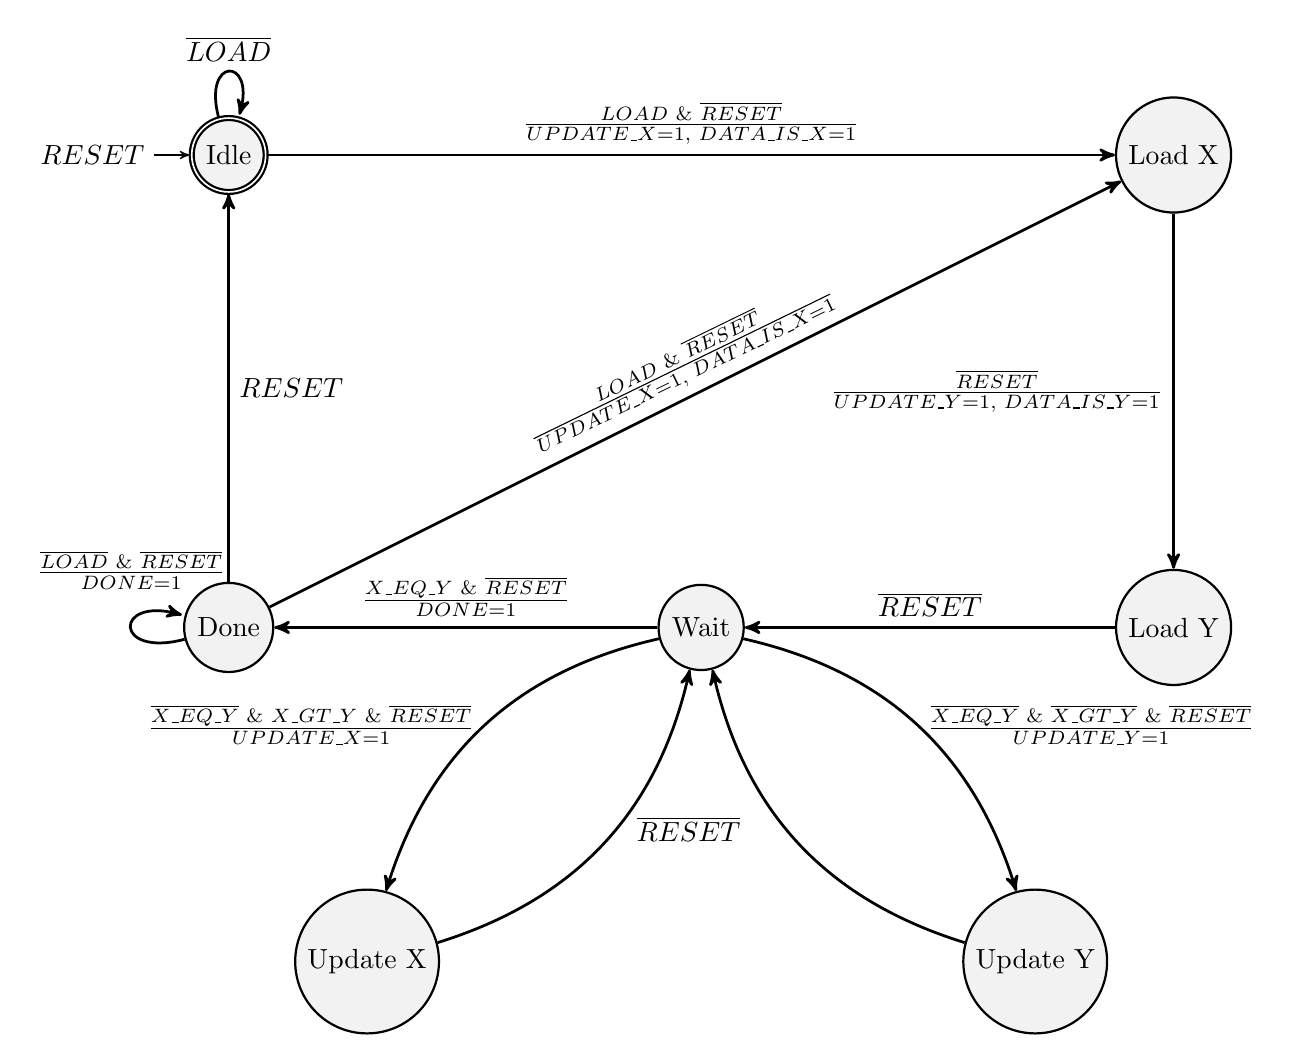
\begin{tikzpicture}[initial text=$RESET$]
	\node[state, initial, accepting] (Idle) {Idle};
	\node[state, below of=Idle] (Done) {Done};
	\node[state, right of=Done] (Wait) {Wait};
	\node[state, right of=Wait] (Load Y) {Load Y};
	\node[state, above of=Load Y] (Load X) {Load X};
	\node[state, below left of=Wait] (Update X) {Update X};
	\node[state, below right of=Wait] (Update Y) {Update Y};
	\draw[->, line width=0.35mm]
		(Idle) edge[loop above] node{$\overline{LOAD}$} (Idle)
		(Idle) edge[above] node{$\frac{LOAD \text{ \& }\overline{RESET}}{UPDATE\_X=1\text{, }DATA\_IS\_X=1}$} (Load X)
		(Load X) edge[left] node{$\frac{\overline{RESET}}{UPDATE\_Y=1\text{, }DATA\_IS\_Y=1}$} (Load Y)
		(Load Y) edge[above] node[]{$\overline{RESET}$} (Wait)
		(Wait) edge[bend right, left] node{$\frac{\overline{X\_EQ\_Y}\text{ \& }X\_GT\_Y \text{ \& }\overline{RESET}}{UPDATE\_X=1}$} (Update X)
		(Update X) edge[bend right, right] node[xshift=8, yshift=5]{$\overline{RESET}$} (Wait)
		(Wait) edge[bend left, right] node{$\frac{\overline{X\_EQ\_Y}\text{ \& }\overline{X\_GT\_Y}\text{ \& }\overline{RESET}}{UPDATE\_Y=1}$} (Update Y)
		(Update Y) edge[bend left, left] node{} (Wait)
		(Wait) edge[above] node{$\frac{X\_EQ\_Y\text{ \& }\overline{RESET}}{DONE=1}$} (Done)
		(Done) edge[loop left, above] node[yshift=10]{$\frac{\overline{LOAD}\text{ \& }\overline{RESET}}{DONE=1}$} (Done)
		(Done) edge[right] node{$RESET$} (Idle)
		(Done) edge[above] node[rotate=26]{$\frac{LOAD\text{ \& }\overline{RESET}}{UPDATE\_X=1\text{, }DATA\_IS\_X=1}$} (Load X);
\end{tikzpicture}
\caption{Mealy Finite State Machine} \label{FSM}
\end{figure}

The addition of the \textit{Done} state is what specifically allows for the \textbf{DONE} signal to be asserted once a calculation has completed. One thing to note about this FSM is that the \textit{Update X} and \textit{Update Y} states are somewhat superfluous because the outputs are asserted on the transitions themselves. However, I kept these states inside the FSM to allow for the datapath to perform any necessary arithmetic (in this case $x-y$ and $y-x$) without worrying about the time required to properly evaluate \textbf{X\_EQ\_Y} and \textbf{X\_GT\_Y}. I did remove these states in my first design of this project, but it resulted in $x$ and $y$ being updated when they were not supposed to be, underflowing the result and timing out the simulation.

\subsection{Datapath}
The only required change (relative to the starting DP1 code) to my datapath was to utilize two subtractors to compute $x-y$ and $y-x$ simultaneously. This affected my implementation by requiring one less input to the datapath module (because there is no need to select which values to subtract). Otherwise, the GCD algorithm itself was implemented identically.

\subsection{Problems}
I first encountered a problem when the \Vivado -generated inputs and outputs to my modules -- those specified at the creation of the module itself -- were not given the keyword \textbf{signal}. This resulted in me assuming it was superfluous, and thus my simulation failed for (seemingly) random reasons. I eventually realized the IDE did not insert the \textbf{signal} keyword, but it was necessary nonetheless.

One more error I made was failing to define the vector size for the \textbf{gcd\_result} signal. This was not identified by \Vivado as an error, but resulting in a simulation in which only bit 0 of the vector was being utilized by my datapath, and thus the algorithm was not performing as expected.

The final problem I encountered was due to me incorrectly creating the testbench \SV file, and I utilized it as a design source instead of exclusively a simulation source. This only became relevant when performing my post-synthesis simulation, and was inevitably fixed by treating that file as just a simulation source.

As I mentioned previously, attempting to implement the FSM without the \textit{Update X} and \textit{Update Y} states resulted in improper behavior. In the post-synthesis simulation the previous output of $UPDATE\_X=1$ resulted in the sequential logic of the datapath module updating $x$ and $y$ (as at the clock-edge the output was still high, as the state transition hadn't completed) one too many times, and underflowing. This was only rectified by adding those states, slowing down the algorithm -- but since we were not given specific timing requirements, this implementation is adequate.

\section{Simulations}
\subsection{Behavioral Simulation}
Due to the length of the simulation, I captured the Behavioral Simulation in four parts, shown below. My simulation was done with an input $x=63$, and $y=12$.

\begin{figure}[H]
\centering
\includegraphics[width=\textwidth]{Project_2/Outputs/Sim1.PNG}
\caption{First 700 nanoseconds of the Behavioral Simulation.}
\label{fig:behav-sim1}
\end{figure}

\begin{figure}[H]
\centering
\includegraphics[width=\textwidth]{Project_2/Outputs/Sim2.PNG}
\caption{Second 700 nanoseconds of the Behavioral Simulation.}
\label{fig:behav-sim2}
\end{figure}

\begin{figure}[H]
\centering
\includegraphics[width=\textwidth]{Project_2/Outputs/Sim3.PNG}
\caption{Third 700 nanoseconds of the Behavioral Simulation.}
\label{fig:behav-sim3}
\end{figure}

\begin{figure}[H]
\centering
\includegraphics[width=\textwidth]{Project_2/Outputs/Sim4.PNG}
\caption{Final 500 nanoseconds of the Behavioral Simulation.}
\label{fig:behav-sim4}
\end{figure}

As evident in the behavioral simulation, each relevant module functions as expected. After approximately 300 nanoseconds of resetting, the FSM transitions between the \textbf{Idle}, \textbf{Load X}, and \textbf{Load Y} states in three sequential clock cycles.

Afterwards, the changing values of \textbf{x} and \textbf{y} can be seen in the following pictures. The two values decrease in their respective states, until they're equal with a value of $3$ (the correct result). Then, the \textbf{done} signal is asserted, followed by \textbf{reset}. 

\subsection{Post-Synthesis Simulation}
I was able to capture the post-synthesis simulation with a single image, and the result exactly matches those of my behavioral simulation. Even the time it takes for the \textbf{done} signal to be asserted was identical to my previous simulation (which is good!).

\begin{figure}[H]
\centering
\includegraphics[width=\textwidth]{Project_2/Outputs/Post-Synth-Sim1.PNG}
\caption{Complete Post-Synthesis Simulation.}
\label{fig:post-synth-sim}
\end{figure}

\section{Synthesis Report}
\lstinputlisting[breaklines, nolol=True]{Project_2/Outputs/gcd_core.vds} % Read external file

\section{Source Code}
\begin{mdframed}[backgroundcolor=code-gray, roundcorner=10pt, innerleftmargin=15, innertopmargin=5, innerbottommargin=5]	
\lstinputlisting[breaklines, language=Verilog, caption=Finite State Machine Module, tabsize=2, label={lst:fsm-module}]{Project_2/Outputs/fsm.sv}
\end{mdframed}
	
\begin{mdframed}[backgroundcolor=code-gray, roundcorner=10pt, innerleftmargin=15, innertopmargin=5, innerbottommargin=5]	
\lstinputlisting[breaklines, language=Verilog, caption=Datapath Module, tabsize=2, label={lst:dp-module}]{Project_2/Outputs/dp.sv}
\end{mdframed}
	
\begin{mdframed}[backgroundcolor=code-gray, roundcorner=10pt, innerleftmargin=15, innertopmargin=5, innerbottommargin=5]	
\lstinputlisting[breaklines, language=Verilog, caption=GCD Core Module, tabsize=2, label={lst:gcd-core-module}]{Project_2/Outputs/gcd_core.sv}
\end{mdframed}

\begin{mdframed}[backgroundcolor=code-gray, roundcorner=10pt, innerleftmargin=15, innertopmargin=5, innerbottommargin=5]	
\lstinputlisting[breaklines, language=Verilog, caption=Testbench, tabsize=2, label={lst:testbench}]{Project_2/Outputs/testbench.sv}
\end{mdframed}

\end{document}